\documentclass[landscape,a0paper]{baposter}

\usepackage[vlined]{algorithm2e}
\usepackage{times}
\usepackage{calc}
\usepackage{url}
\usepackage{graphicx}
\usepackage{amsmath}
\usepackage{amssymb}
\usepackage{relsize}
\usepackage{multirow}
\usepackage{booktabs}

\usepackage{graphicx}
\usepackage{multicol}
\usepackage[T1]{fontenc}
\usepackage{ae}
\begin{document}
\begin{poster}
{
columns=4,
borderColor=green,
headerheight=0.18\textheight,
background = none,
bgColorOne=white,
borderColor=green!60!yellow,
headerColorOne =  green!60!yellow,
headerColorTwo = white,
textborder=roundedright,
headerborder=open,
headershape=rounded,
headershade=plain,
boxshade=none,
}
{
\includegraphics[height=0.08\textheight]{cuda.jpeg}
}
{Gate Level Event-Driven Simulation using GPGPUs with CUDA}
{Se\c{c}kin Sava\c{s}\c{c}\i , Alper \c{S}en \\
\texttt{\{seckin.savasci, alper.sen\} @boun.edu.tr}}
{
	\includegraphics[height=0.15\textheight]{2000px-boun.png}
}

\headerbox{Why do we need simulation?}{name=whysimulation,column=0,row=0,span=1}{
%%%%%%%%%%%%%%%%%%%%%%%%%%%%%%%%%%%%%%%%%%%%%%%%%%%%%%%%%%%%%%%%%%%%%%%%%%%%%%
\textbf{More than half} of the effort in the design phase goes for verification and validation of the design! \\ 
Performance for gate level netlist simulation is extremely low; typically it takes \textbf{days} to validate a particular design. But netlist simulation performance is quite significant since short times-to-market limit the coverage that can be achieved in verification. Thus, faster verification methods are needed to improve coverage.
}



\headerbox{Simulation 101}{name=simulation101,below=whysimulation}{
%%%%%%%%%%%%%%%%%%%%%%%%%%%%%%%%%%%%%%%%%%%%%%%%%%%%%%%%%%%%%%%%%%%%%%%%%%%%%%
\centering \includegraphics[height=0.12\textheight]{simfd.png}

\subsection*{Simulation at a glance}
\begin{enumerate}
\item get the inputs
\item process the inputs
\item get the outputs
\end{enumerate}
\subsection*{Simulation Types}
\begin{enumerate}
\item \textbf{Straightforward :} Simulate all sequentially!
\item \textbf{Parallel :} Simulate parallel if you can!
\item \textbf{Event-Driven : } Simulate parts if needed! 
\end{enumerate}
\centering 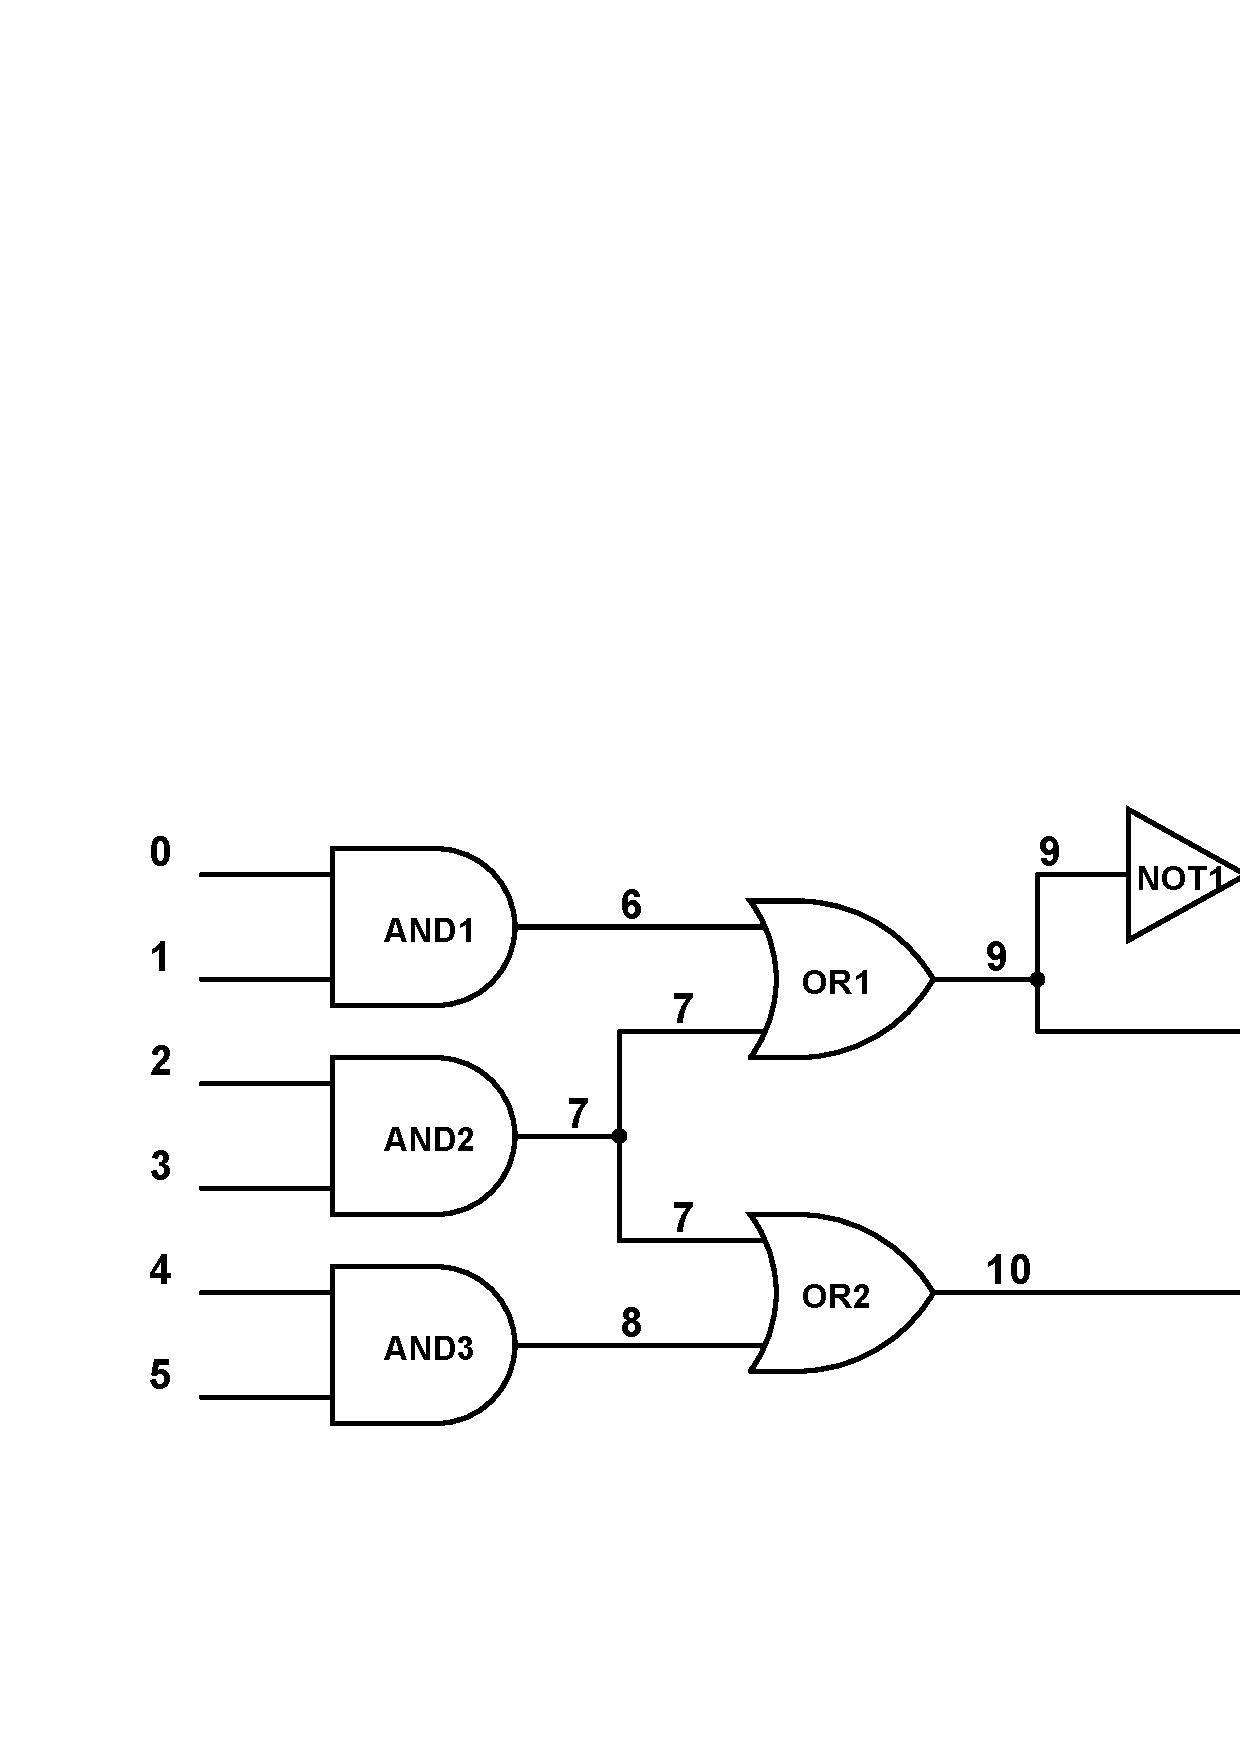
\includegraphics[height=0.15\textheight]{senior_demo.png}
}



  
  

\headerbox{Why CUDA?}{name=whycuda,column=1}{
%%%%%%%%%%%%%%%%%%%%%%%%%%%%%%%%%%%%%%%%%%%%%%%%%%%%%%%%%%%%%%%%%%%%%%%%%%%%%%
\emph{CUDA[1] stands for \emph{Compute Unified Device Architecture}. It is a parallel programming platform and a programming model created by NVIDIA. It enables programmers to develop programs using massively parallel architecture of GPUs.}
\begin{itemize}
\item[+] Easy to learn
\item[+] C + some gpu related calls
\item[+] Easily wrappable for C++
\item[-] Architecture dependent
\item[-] NVDIA only
\item[-] Host-Device distance
\end{itemize}
}
  

\headerbox{CUDA 101}{name=cuda101,column=1,span=1,below=whycuda}{
%%%%%%%%%%%%%%%%%%%%%%%%%%%%%%%%%%%%%%%%%%%%%%%%%%%%%%%%%%%%%%%%%%%%%%%%%%%%%%
\begin{itemize}
\item CUDA version 5.0 , currently being developed for full C++ support
\item Have helper libraries like Thrust[2], CUBLAS[3]
\item Atomic operations for integer and float
\item Multiple GPU support
\item Same naming : cudaMalloc(), cudaMemcpy() 
\item OpenGL integration
\item Several Built-in Memory types: Global, shared, texture
\item function$<<<blocks,threads>>>$(args...)
\end{itemize}
\centering \includegraphics[height=0.15\textheight]{cuda_tbg.jpg}
  }

\headerbox{Contributions}{name=contributions,column=3,span=1}{
%%%%%%%%%%%%%%%%%%%%%%%%%%%%%%%%%%%%%%%%%%%%%%%%%%%%%%%%%%%%%%%%%%%%%%%%%%%%%%
\begin{itemize}
\item \textbf{Circuit Generator} \\ A random circuit generator for our own circuit format
\item \textbf{Run Generator} \\ A random run generator that feeds the simulation with inputs in each timestep
\item \textbf{Sequential Event-Driven Circuit Simulator(Enigma)} \\ A sequential circuit simulator written in C++
\item \textbf{Parallel Event-Driven Circuit Simulator(Meepo)} \\ Our project goal, parallelized version of Enigma simulator, 
with the help of CUDA
\end{itemize}
}

\headerbox{Simulation Diagram}{name=diagram,column=2,span=1}{
%%%%%%%%%%%%%%%%%%%%%%%%%%%%%%%%%%%%%%%%%%%%%%%%%%%%%%%%%%%%%%%%%%%%%%%%%%%%%%
\centering \includegraphics[height=0.25\textheight]{diagram.png}
}
\headerbox{Results}{name=results,column=2,span=2,below=contributions}{
%%%%%%%%%%%%%%%%%%%%%%%%%%%%%%%%%%%%%%%%%%%%%%%%%%%%%%%%%%%%%%%%%%%%%%%%%%%%%%
Results demonstrates up to 6x speed-up in simulation. These results are obtained by simulating several circuits with random structures for one hundred input vectors.
\centering \begin{tabular}{| r | r | r | r |}

\hline                        
Gates & Enigma(sec) & Meepo(sec) & Speed-up \\ \hline 
1000 & 2.08 & 0.943 & 2.206 \\ \hline
2000 & 6.053 & 1.658  & 3.651 \\ \hline
3000 & 12.438 & 2.915 & 4.267 \\ \hline
5000 & 32.246 & 6.363  & 5.068 \\ \hline
10000 & 118.059 & 20.907 & 5.647 \\ \hline
20000 & 493.285 & 85  & 5.803 \\ \hline
30000 & 1060.34 & 181.785  & 5.833 \\ \hline
\end{tabular}

\begin{tabular}{c c}
\includegraphics[height=0.15\textheight]{graph1.png} & \includegraphics[height=0.15\textheight]{graph2.png} \\
\end{tabular}

  }

\headerbox{References}{name=refs,column=2,span=2,below=results}{
%%%%%%%%%%%%%%%%%%%%%%%%%%%%%%%%%%%%%%%%%%%%%%%%%%%%%%%%%%%%%%%%%%%%%%%%%%%%%%
1 : to get started,please visit developer.nvidia.com/cuda \\
2 : Thrust library aims to provide c++ stl capabilities for CUDA, see thrust.github.com \\
3 : CUBLAS is a port of famous scientif package BLAS, see developer.nvidia.com/cublas \\
}


\end{poster}
\end{document}